NetChain \cite{netchain} is an in-network solution for coordination services, such as distributed locking, barriers, etc.
All these services are realized on top of a strongly-consistent and fault-tolerant key-value store, which is entirely implemented in the network data plane.
The network device in charge of storing the distributed store is a programmable switch: this brings an obvious limitation in terms of storage size, that makes NetChain \cite{netchain} an acceptable solution only when a small amount of critical data must be stored in the network data plane, e.g., coordination services.\par
NetChain \cite{netchain} can process queries entirely in the network data plane, causing the end-to-end latency to drop from multiple RTTs to as little as half of one RTT since servers are not involved in query processing anymore.

\subsubsection{Details}
\paragraph{Packets}
Custom UDP packets are used for queries, containing fields like \textit{operation}, \textit{key} and \textit{value}.
Read and write queries only involve the network data plane, while insert and delete queries involve the network controller to set up entries in switch tables and to perform garbage collection, respectively.

\begin{figure}[!htb]
    \centering
        % trim = left, bottom, right, top
        \includegraphics[page=5, clip, trim=3.6cm 0.7cm 10cm 4.15cm, width=0.8\textwidth]{figures/analysis/inp/presentation.pdf}
    \caption{NetChain's \texorpdfstring{\cite{netchain}}{} basic topology and entities}
\end{figure}

This is acceptable since coordination services usually perform read and write queries on already-existing objects, e.g., locks.
Each switch has its own IP address, and packet headers contain the list of addresses of switches to be traversed, allowing those to properly forward packets to the their successors (from head to tail for write queries and the opposite for read queries).
\begin{figure}[!htb]
    \centering
        % trim = left, bottom, right, top
        \includegraphics[page=8, clip, trim=6.5cm 0.1cm 6.4cm 0.1cm, width=1.00\textwidth]{figures/analysis/inp/presentation.pdf}
    \caption{Messages exchanged during a NetChain \texorpdfstring{\cite{netchain}}{} instance execution}
\end{figure}
This list of IP addresses is inserted by the client (a NetChain \cite{netchain} agent).

\paragraph{Consistency}
A variant of Chain Replication \cite{chainreplication} is used in the data plane to handle read and write queries and to ensure strong consistency, while switches reconfiguration is handled by the network control plane.
The main difference with the standard Chain Replication \cite{chainreplication} protocol is that objects are stored on programmable switches instead of servers.
Switches are logically connected together in order to form an oriented chain.

\begin{figure}[!htb]
    \centering
        % trim = left, bottom, right, top
        \includegraphics[page=6, clip, trim=3.6cm 0.7cm 3.2cm 4.15cm, width=1.00\textwidth]{figures/analysis/inp/presentation.pdf}
    \caption{NetChain's \texorpdfstring{\cite{netchain}}{} extended topology}
\end{figure}

Read queries are processed by the \textit{tail} switch while write queries are sent to the \textit{head} switch, which will forward the updated state to the rest of the chain.

\begin{figure}[!htb]
    \centering
        % trim = left, bottom, right, top
        \includegraphics[page=7, clip, trim=3.6cm 0.7cm 3.6cm 4.15cm, width=1.00\textwidth]{figures/analysis/inp/presentation.pdf}
    \caption{NetChain's \texorpdfstring{\cite{netchain}}{} logical communication pattern}
\end{figure}

The key-value store is partitioned amongst \textit{virtual nodes} using consistent hashing, mapping keys to a hash ring.
Each ring segment is stored by $f + 1$ virtual nodes allocated on different physical switches, hence tolerating faults involving up to $f$ switches.

\subsubsection{Implementation}
The network data plane has been programmed in P4 \cite{p4} while the controller has been coded in Python, it runs on a server and communicates with switches through the standard Python RPC library.
Switches agents are Python processes who run in the switch OS. Some P4 \cite{p4} drawbacks were already discussed in \cref{p4_drawbacks}.\par
The out-of-order UDP delivery problem is resolved by adding sequence numbers to write queries, hence serializing those operations, while the loss of packets is coped by \textit{client-side retries} based on timeouts.

\subsubsection{Minimum system requirements}
Network devices must form a chain of length $f + 1$ in order to tolerate $f$ failures. The client must include the list of IP addresses of all the $f + 1$ switches to be traversed in each query packet header (from head to tail for write queries and the opposite
for read queries; storing the entire backward list for read queries is only necessary in case of tail failures).\par
Network devices must dedicate some local storage to NetChain \cite{netchain}: more specifically, they need to store a
\begin{mylist}
    \item register array to store values and a
    \item match-action table to store the keys' location in the register array and the corresponding action to be performed
\end{mylist}.
The solution requires that the system has a centralized \gls{sdn} controller connected to all switches.
The \gls{sdn} controller must handle switches reconfigurations.

\subsubsection{Conclusions}
NetChain \cite{netchain} inventors state that the on-chip memory of programmable switches in enough for coordination services.
Assuming a $\SI{10}{\mega\byte}$ partition allocated on each NetChain \cite{netchain} switch, a data center with 100 switches can provide a $(\SI{10}{\mega\byte} \cdot 100) / 3 = \SI{333}{\mega\byte}$ storage with a replication factor of three: that would be enough for the average number of files (22k, from 0 to 1 byte) managed by a typical Chubby \cite{chubby} lock service instance, as cited by Google in their corresponding paper.
Likewise, inventors claim that switches total memory is enough for a distributed locking system: assuming $\SI{30}{\byte}$ locks, the previously-mentioned example would be capable of storing $\SI{333}{\mega\byte} / \SI{30}{\byte} = 10M$ concurrent locks.